% Copy selected PDFs into figures/. Use landscape/full-page placement to preserve >=9 pt labels.
% See print_ready_maps.pdf and print_audit.json for verified page sizes.

\begin{figure}[htbp]
\centering
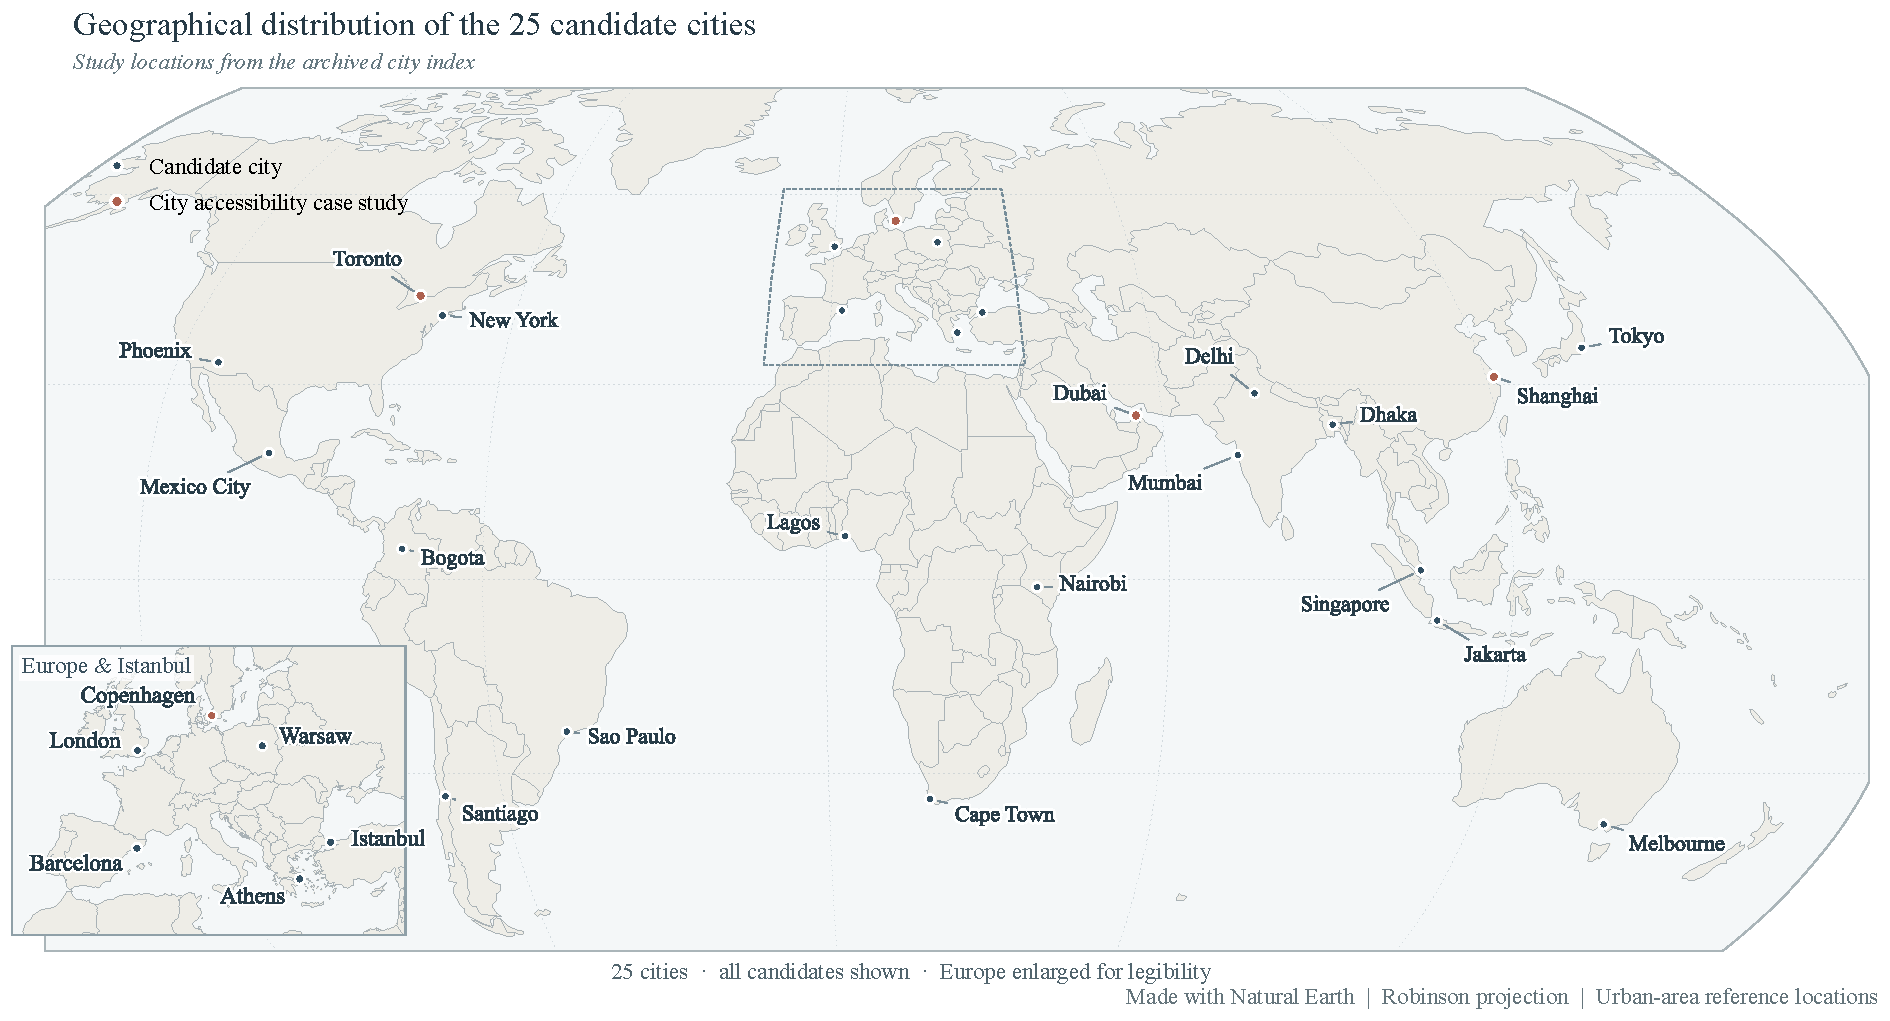
\includegraphics[width=\linewidth]{figures/01_global_candidates.pdf}
\caption{Geographical distribution of the 25 candidate cities.}
\label{fig:01_global_candidates}
\end{figure}

\begin{figure}[htbp]
\centering
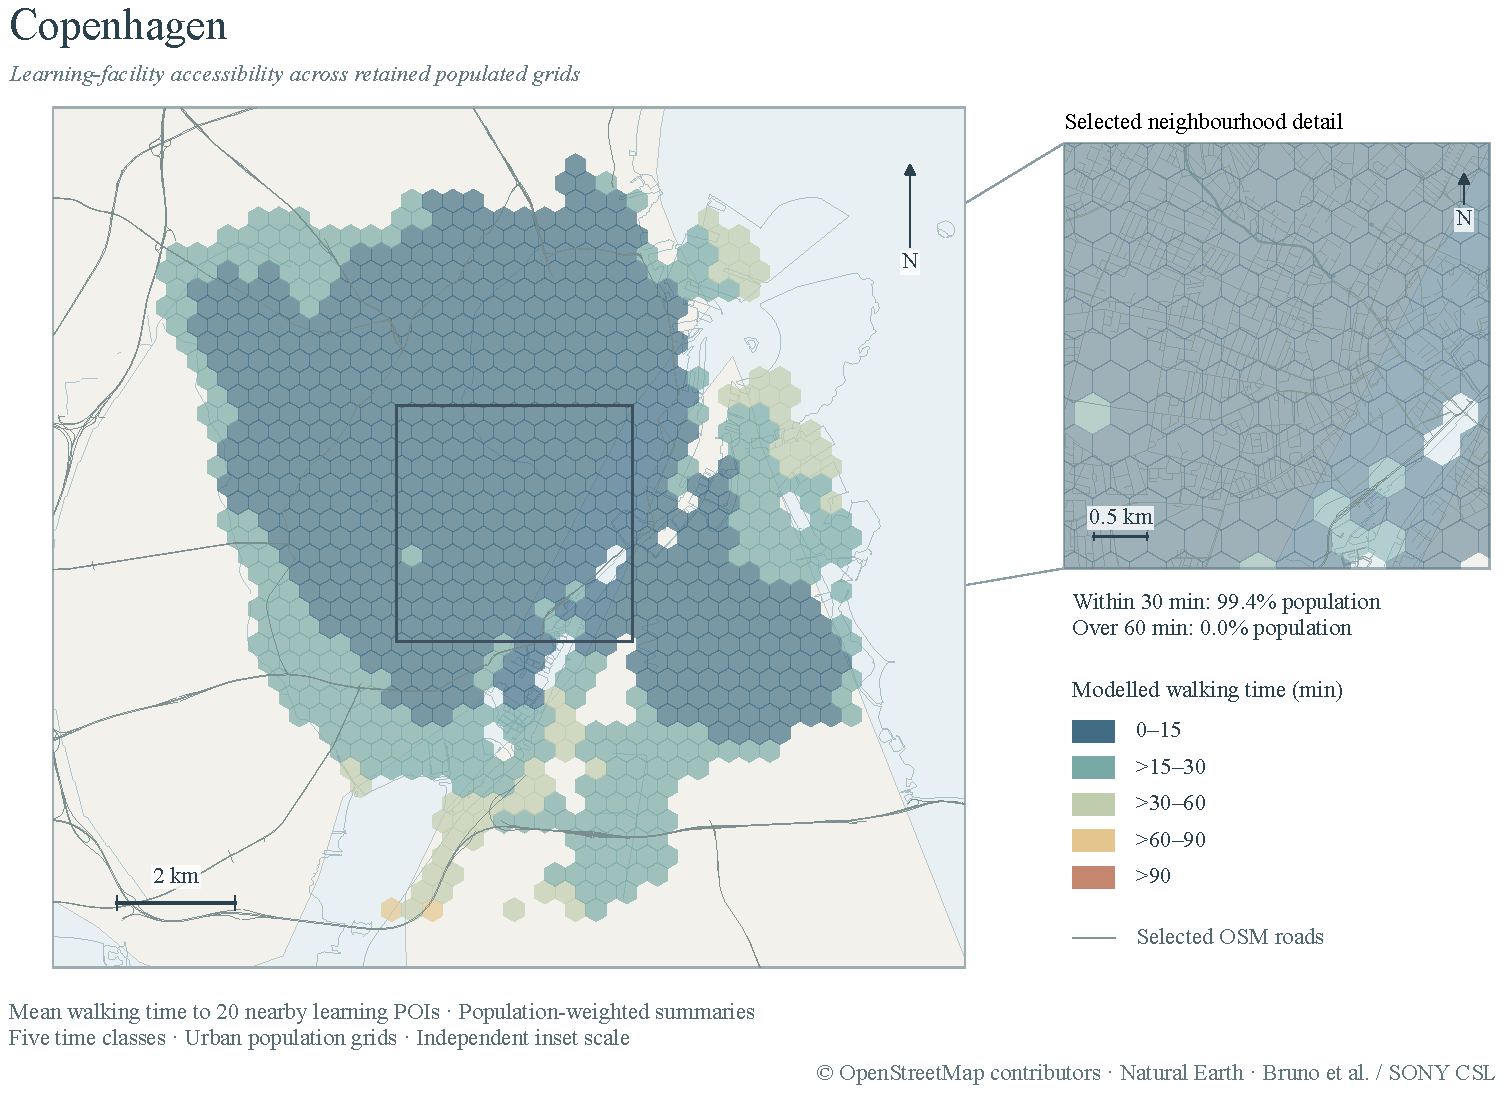
\includegraphics[width=\linewidth]{figures/02_copenhagen_access.pdf}
\caption{Learning-facility walking accessibility in Copenhagen, using archived modelled mean travel times to the nearest 20 Learning POIs and retained all-age population grids. Grey roads provide current OpenStreetMap geographical context for the archived accessibility estimates. The full populated-grid footprint and selected detail use separate scales. Coverage follows the source urban-area dataset.}
\label{fig:02_copenhagen_access}
\end{figure}

\begin{figure}[htbp]
\centering
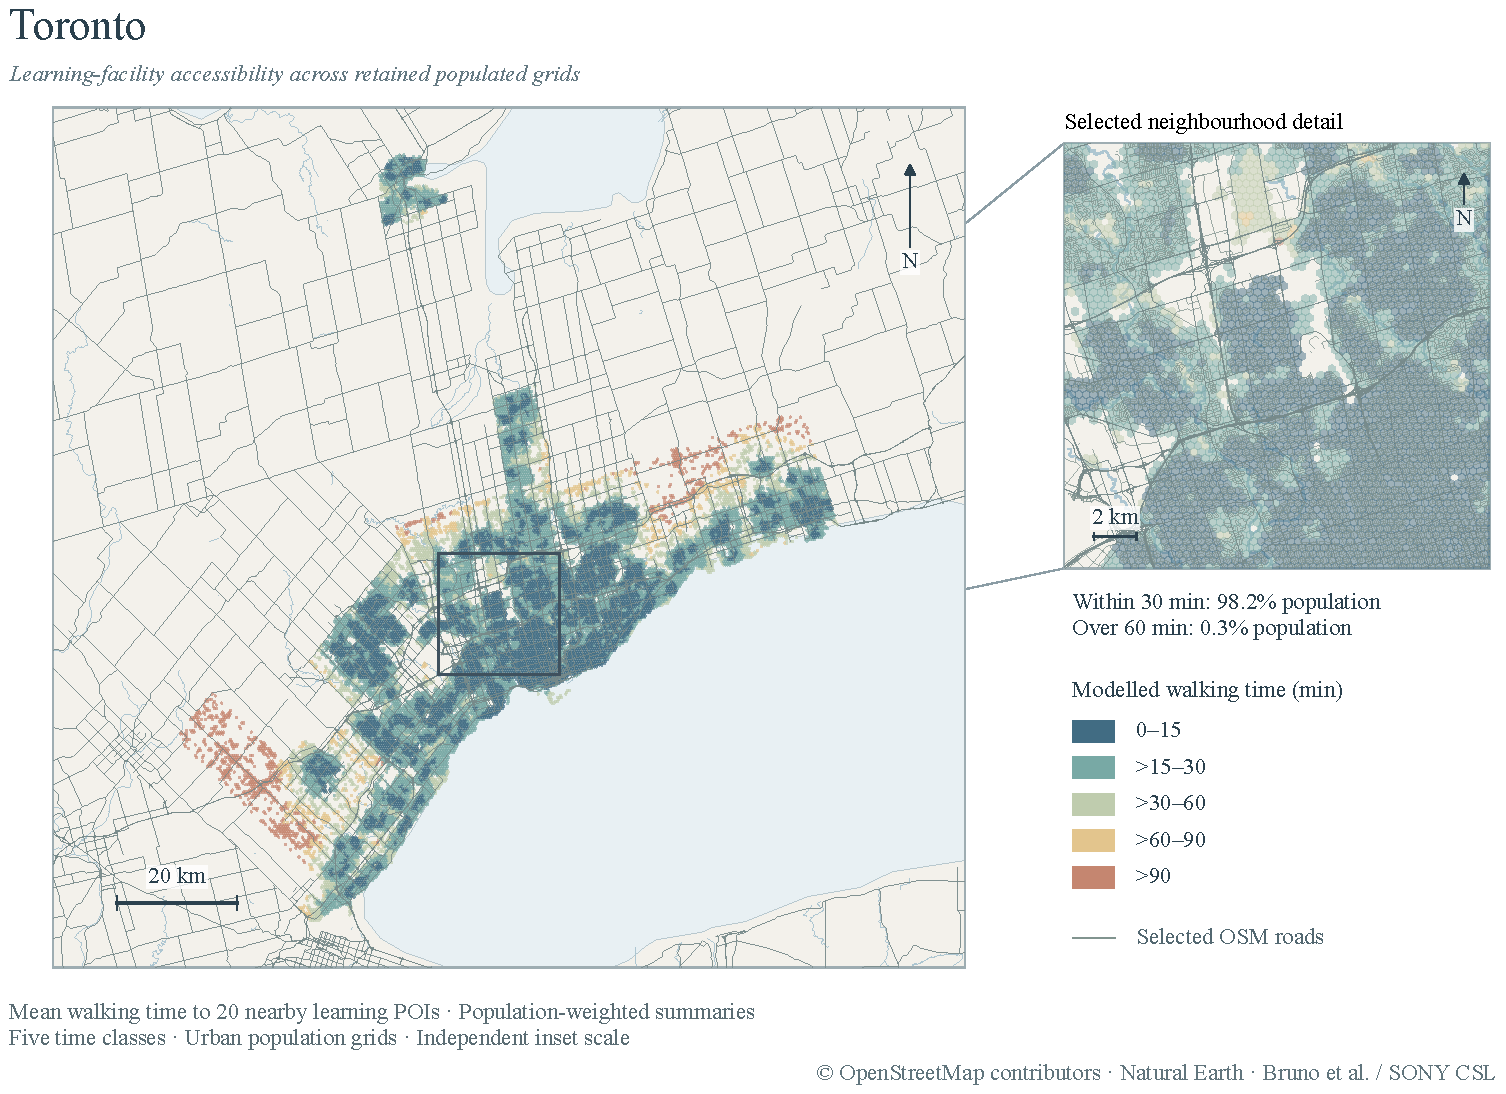
\includegraphics[width=\linewidth]{figures/03_toronto_access.pdf}
\caption{Learning-facility walking accessibility in Toronto, using archived modelled mean travel times to the nearest 20 Learning POIs and retained all-age population grids. Grey roads provide current OpenStreetMap geographical context for the archived accessibility estimates. The full populated-grid footprint and selected detail use separate scales. Coverage follows the source urban-area dataset.}
\label{fig:03_toronto_access}
\end{figure}

\begin{figure}[htbp]
\centering
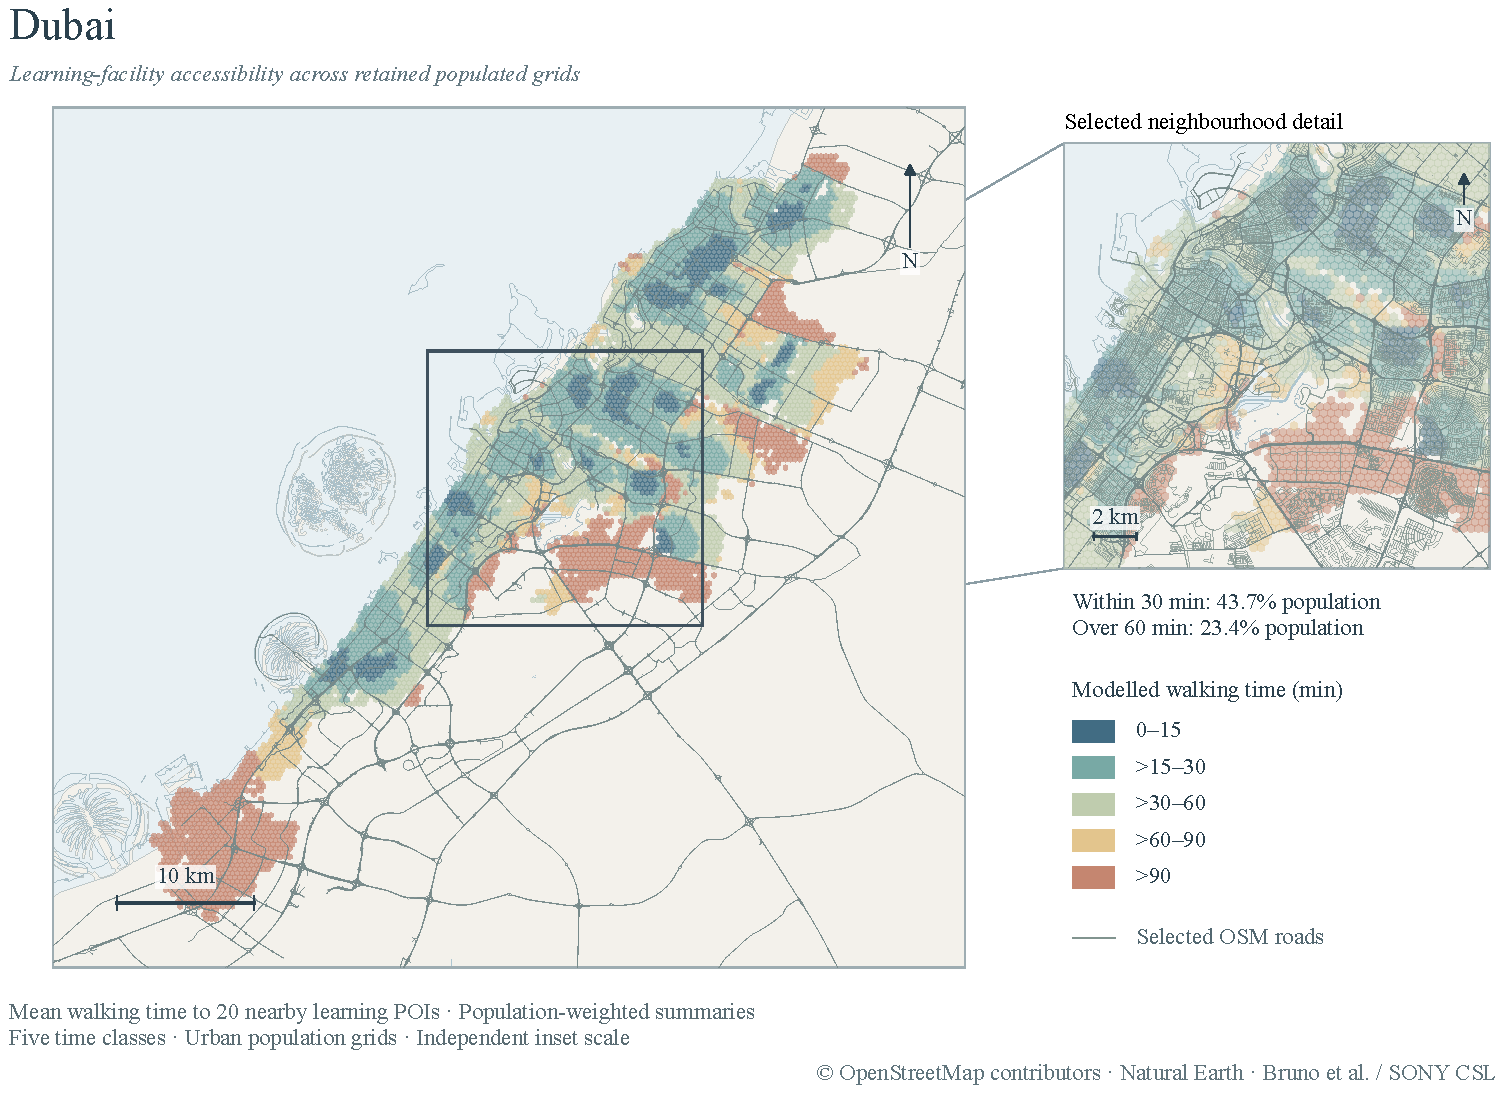
\includegraphics[width=\linewidth]{figures/04_dubai_access.pdf}
\caption{Learning-facility walking accessibility in Dubai, using archived modelled mean travel times to the nearest 20 Learning POIs and retained all-age population grids. Grey roads provide current OpenStreetMap geographical context for the archived accessibility estimates. The full populated-grid footprint and selected detail use separate scales. Coverage follows the source urban-area dataset.}
\label{fig:04_dubai_access}
\end{figure}

\begin{figure}[htbp]
\centering
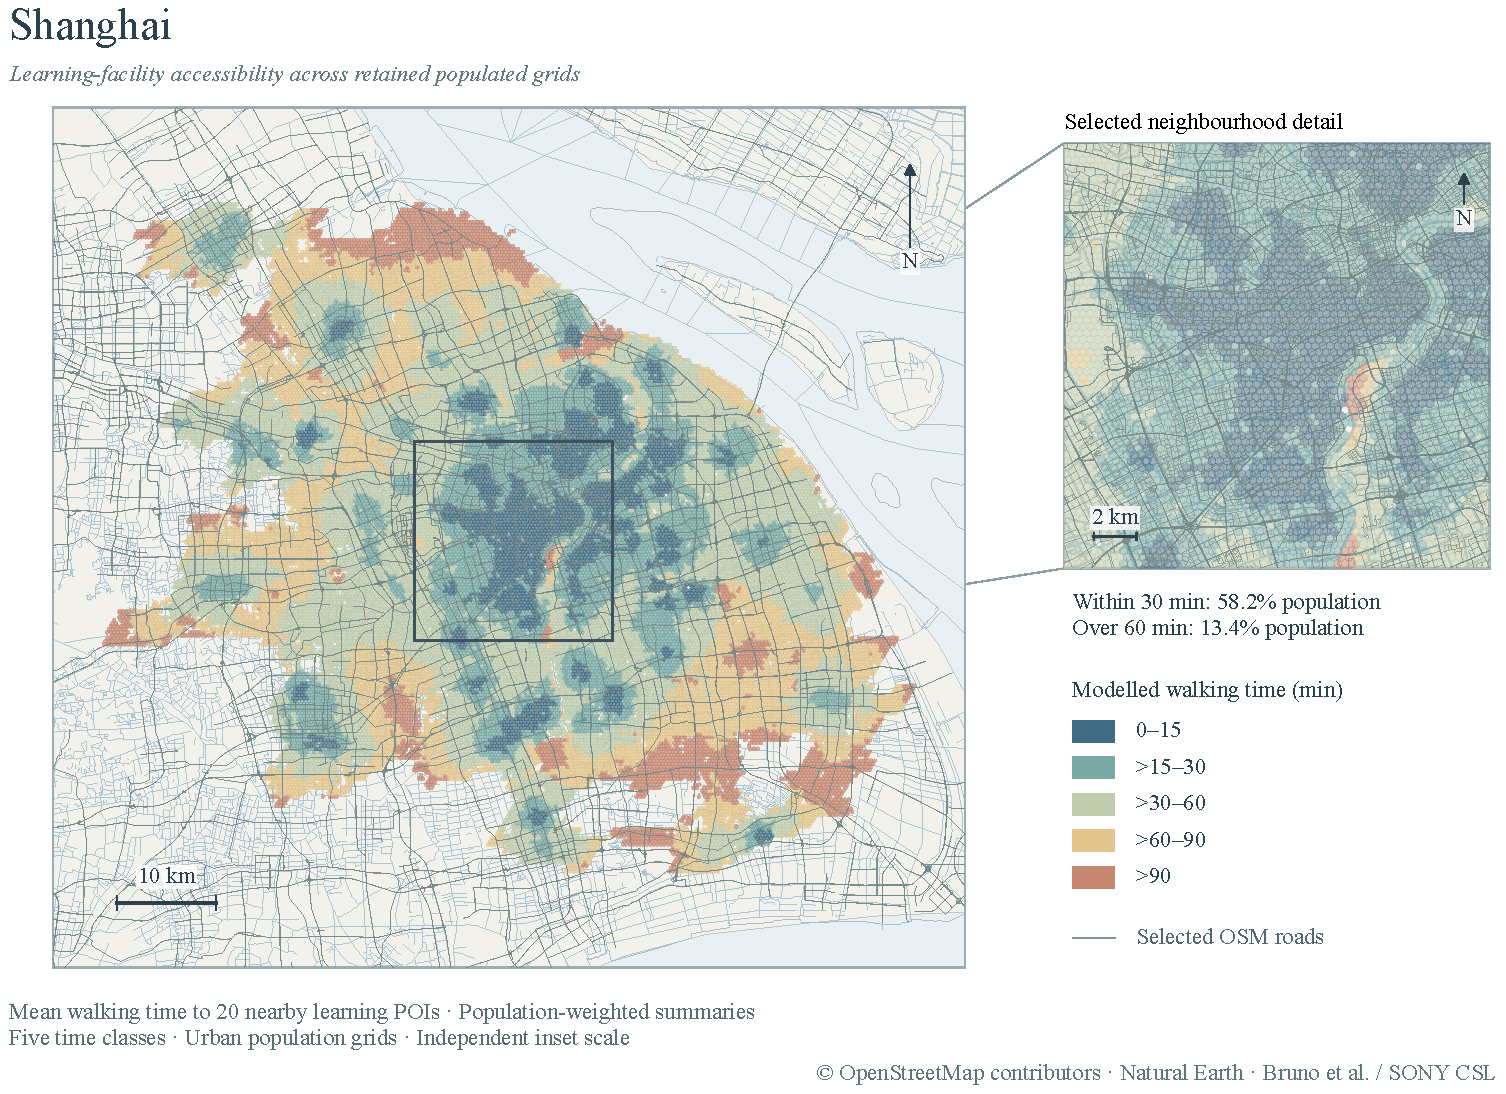
\includegraphics[width=\linewidth]{figures/05_shanghai_access.pdf}
\caption{Learning-facility walking accessibility in Shanghai, using archived modelled mean travel times to the nearest 20 Learning POIs and retained all-age population grids. Grey roads provide current OpenStreetMap geographical context for the archived accessibility estimates. The full populated-grid footprint and selected detail use separate scales. Coverage follows the source urban-area dataset.}
\label{fig:05_shanghai_access}
\end{figure}

\begin{figure}[htbp]
\centering
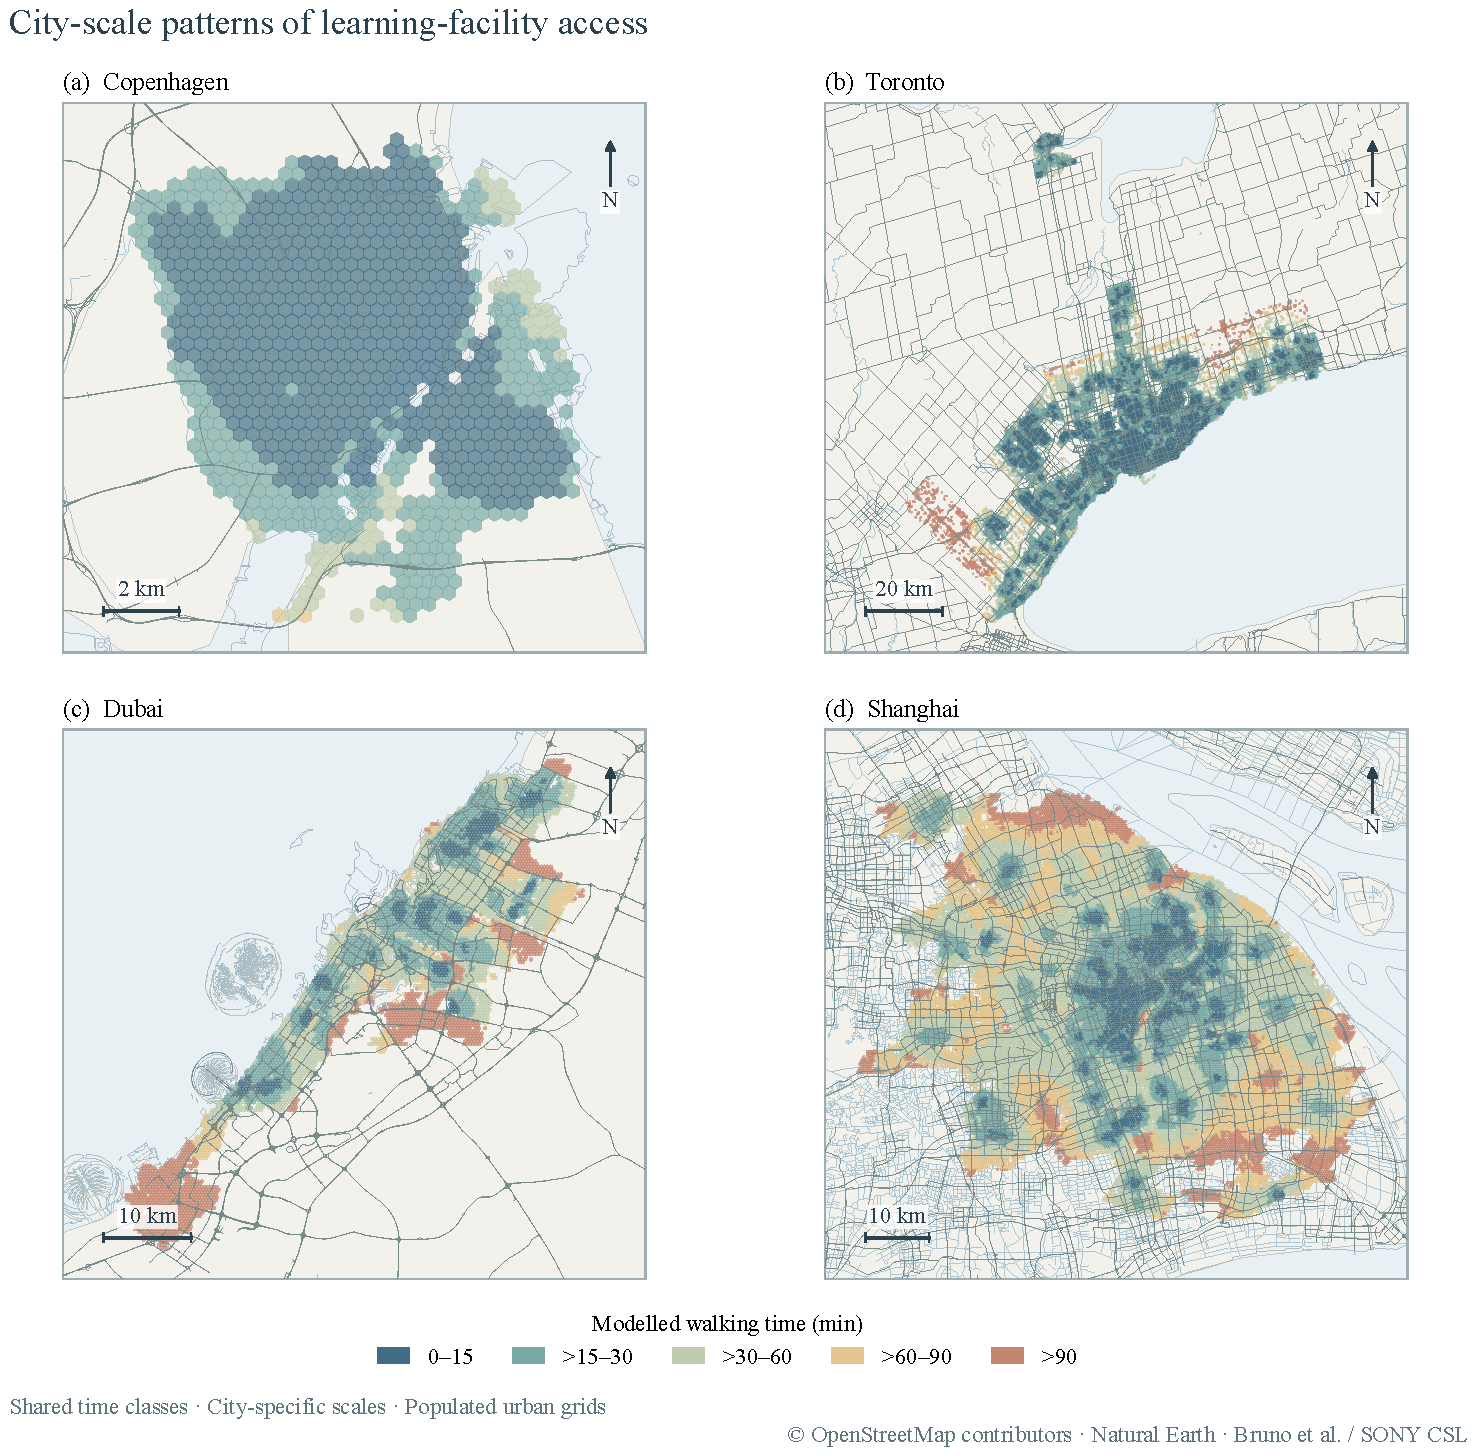
\includegraphics[width=\linewidth]{figures/06_city_access_comparison.pdf}
\caption{Learning-facility walking accessibility across four cities, using common time classes and city-specific map scales.}
\label{fig:06_city_access_comparison}
\end{figure}